\pdfoutput=1
\documentclass[a4paper,pdflatex,ja=standard]{bxjsarticle}

% ---Setting about the geometry of the document----
% \usepackage{a4wide}
% \pagestyle{empty}

% ---Physics and Math Packages---
\usepackage{amssymb,amsfonts,amsthm,mathtools}
\usepackage{physics,braket,bm}

% ---underline---
\usepackage{ulem}

% --- sorround the texts or equations
% \usepackage{fancybox,ascmac}

% ---settings of theorem environment---
% \usepackage{amsthm}
% \theoremstyle{definition}

% ---settings of proof environment---
% \renewcommand{\proofname}{\uline{\textbf{証明}}}
% \renewcommand{\qedsymbol}{$\blacksquare$}

% ---Ignore the Warnings---
\usepackage{silence}
\WarningFilter{latexfont}{Some font shapes,Font shape}

% ---Insert the figure (If insert the `draft' at the option, the process becomes faster)---
\usepackage{graphicx}
% \usepackage{subcaption}

% ----Add a link to a text---
\usepackage{url}
\usepackage{xcolor,hyperref}
\hypersetup{colorlinks=true,citecolor=orange,linkcolor=blue,urlcolor=magenta}
\usepackage{bxcjkjatype}

% ---Tikz---
\usepackage{tikz,pgf,pgfplots,circuitikz}
\pgfplotsset{compat=1.15}
\usetikzlibrary{intersections,arrows.meta,angles,calc,3d,decorations.pathmorphing}

% ---Add the section number to the equation, figure, and table number---
\makeatletter
   \renewcommand{\theequation}{\thesubsection.\arabic{equation}}
   \@addtoreset{equation}{subsection}
   
   \renewcommand{\thefigure}{\thesection.\arabic{figure}}
   \@addtoreset{figure}{section}
   
   \renewcommand{\thetable}{\thesection.\arabic{table}}
   \@addtoreset{table}{section}
\makeatother

% ---enumerate---
\renewcommand{\labelenumi}{\arabic{enumi}.}
\renewcommand{\labelenumii}{(\roman{enumii})}
\renewcommand{\labelenumiii}{(\alph{enumiii})}

% ---Index---
% \usepackage{makeidx}
% \makeindex

% ---Fonts---
\renewcommand{\familydefault}{\sfdefault}

% ---Title---
\title{東京大学\ 平成23年\ 物理学専攻\ 院試\ 解答例}
\author{ミヤネ}
\date{最終更新:\today}

\newcommand{\prb}[2]{
  \phantomsection
  \addcontentsline{toc}{subsection}{問題 #1: #2}
  \subsection*{第#1問\phantom{#2}}
  \setcounter{subsection}{#1}
  \setcounter{equation}{0}
}

\begin{document}

\maketitle

\tableofcontents
\clearpage


\section{数学パート}

\prb{1}{線形代数}

\begin{enumerate}

  \item 

  固有値と固有ベクトルをそれぞれ$\lambda,\ \bm{v}$とすれば$A\bm{v}=\lambda\bm{v}$ですが,$A^2\bm{v}$を考えると,$\lambda^2\bm{v}=\bm{v}$となるので$\lambda=\pm1$.


  \item 

  $C^2=-ABAB=ABBA=E$,$BC+CB=-iBAB-iABB=O$,$CA+AC=-iABA-iAAB=O$.


  \item 

  $D^2=(A+iB)(A-iB)=A^2-B^2+i(AB+BA)=O$.また,もし$D=O$だと仮定すると$A=-iB$となりますが,これは
  \begin{equation}
    AB+BA
    =
    -2i B^2
    \neq 
    0
  \end{equation}
  なので矛盾です.よって,$D\neq O$.


  \item 

  \begin{enumerate}

    \item 

    $D\bm{p}=0$より,$A\bm{p}=-iB\bm{p}$なので
    \begin{equation}
      C\bm{p}
      =
      -iA(iA\bm{p})
      =
      \bm{p}
    \end{equation}
    より,固有値は$1$.また,$\bm{q}=A\bm{p}/2-iB\bm{p}/2=A\bm{p}$に気をつければ
    \begin{equation}
      C\bm{q}
      =
      -iABA\bm{p}
      =
      -A\bm{p}
      =
      -\bm{q}
    \end{equation}より,固有値は$-1$.


    \item 

    互いに異なる固有値に属しているので,$\bm{p}^{\dag}\bm{q}$で直交します.よって,
    \begin{equation}
      a\bm{p}+b\bm{q}=0
    \end{equation}
    が成立しているとすれば,$\bm{p}^{\dag},\ \bm{q}^{\dag}$を左から掛ければ$a=b=0$なので線形独立です.($|\bm{p}|,\ |\bm{q}|$は$0$ではないので.)


  \end{enumerate}
  

  \item 

  \begin{enumerate}

    \item 

    次の行列
    \begin{equation}
      P^{-1}
      =
      \begin{pmatrix}
        \bm{p}^{\dag}/|\bm{p}|^2 \\
        \bm{q}^{\dag}/|\bm{q}|^2 
      \end{pmatrix}
    \end{equation}
    は実際に$P$の逆行列になっているので,$P$は正則です.


    \item 

    $P$は対角化行列なので,
    \begin{equation}
      P^{-1}CP
      =
      \begin{pmatrix}
        1 & 0 \\
        0 & -1
      \end{pmatrix}
    \end{equation}
    です.


    \item 

    $D\bm{p}=0,\ D\bm{q}=2\bm{p}$なので\footnote{
      $D\bm{q}$のほうは
      \begin{align*}
        D\bm{q}
        &=
        \frac{1}{2}(A+iB)(A-iB)\bm{p}
        \nonumber
        \\
        &=
        \frac{1}{2}(2E+2C)\bm{p}
        =
        2\bm{p}
      \end{align*}
      です.
    },
    \begin{align}
      P^{-1}(A+iB)P
      &=
      \begin{pmatrix}
        \bm{p}^{\dag}/|\bm{p}|^2 \\
        \bm{q}^{\dag}/|\bm{q}|^2 
      \end{pmatrix}
      \begin{pmatrix}
        (A+iB)\bm{p} & (A+iB)\bm{q}
      \end{pmatrix}    
      \nonumber
      \\
      &=
      \begin{pmatrix}
        0 & 2 \\
        0 & 0
      \end{pmatrix}
    \end{align}
    となります.一方で,
    \begin{align}
      P^{-1}(A-iB)P
      &=
      \begin{pmatrix}
        \bm{p}^{\dag}/|\bm{p}|^2 \\
        \bm{q}^{\dag}/|\bm{q}|^2 
      \end{pmatrix}
      \begin{pmatrix}
        (A-iB)\bm{p} & (A-iB)\bm{q}
      \end{pmatrix}    
      \nonumber
      \\
      &=
      \begin{pmatrix}
        \bm{p}^{\dag}/|\bm{p}|^2 \\
        \bm{q}^{\dag}/|\bm{q}|^2 
      \end{pmatrix}
      \begin{pmatrix}
        (A-iB)(A\bm{q}) & (A-iB)(A\bm{p})
      \end{pmatrix}    
      =
      \begin{pmatrix}
        \bm{p}^{\dag}/|\bm{p}|^2 \\
        \bm{q}^{\dag}/|\bm{q}|^2 
      \end{pmatrix}
      \begin{pmatrix}
        AD\bm{q} & AD\bm{p}
      \end{pmatrix}          
      \nonumber
      \\
      &=
      \begin{pmatrix}
        \bm{p}^{\dag}/|\bm{p}|^2 \\
        \bm{q}^{\dag}/|\bm{q}|^2 
      \end{pmatrix}
      \begin{pmatrix}
        2\bm{q} & 0
      \end{pmatrix}   
      =
      \begin{pmatrix}
        0 & 0 \\
        2 & 0
      \end{pmatrix}
    \end{align}
    となるので,
    \begin{equation}
      P^{-1}AP
      =
      \begin{pmatrix}
        0 & 1 \\
        1 & 0
      \end{pmatrix}
      ,\ 
      P^{-1}BP
      =
      \begin{pmatrix}
        0 & -i \\
        i & 0
      \end{pmatrix}
    \end{equation}
    となります.


  \end{enumerate}


  \item 

  \begin{equation}
    A
    =
    \begin{pmatrix}
      0 & -i \\
      i & 0 
    \end{pmatrix}
    ,\ 
    B
    =
    \begin{pmatrix}
      0 & 1 \\
      1 & 0 
    \end{pmatrix}
    ,\ 
    C
    =
    \begin{pmatrix}
      -1 & 0\\
      0  & 1 
    \end{pmatrix}
    .
  \end{equation}


\end{enumerate}



\clearpage

\prb{2}{微分方程式}

\begin{enumerate}
  
  \item 

  \begin{enumerate}

    \item 

    $u(x)$を
    \begin{equation}
      u(x)
      =
      \sum_{k=-\infty}^{\infty}
      \tilde{c}_k e^{2\pi ikx}
      ,\ 
      \tilde{c}_k
      =
      \int_0^1
      u(x)e^{-2\pi ikx}
      \dd x
    \end{equation}
    と展開する.すると,境界条件$u(0)=u(1)=0$は
    \begin{equation}
      \sum_{k=-\infty}^{\infty}
      \tilde{c}_k
      =
      0
      \label{bc1}
    \end{equation}
    となります.デルタ関数は
    \begin{equation}
      \delta(x-y)
      =
      \sum_{k=-\infty}^{\infty}
      \tilde{d}_k e^{2\pi ik(x-y)}
    \end{equation}
    と展開できるとすれば,$k\neq 0$では$\tilde{d}_k=1$なので,微分方程式はモード$k$について
    \begin{equation}
      \tilde{c}_k
      =
      -\frac{1}{k^2}e^{-2\pi iky}
      \quad
      (k\neq 0)
    \end{equation}
    と解けることになります.ただし,$\tilde{c}_0$は不定です.したがって,$u(x)$は
    \begin{equation}
      u(x)
      =
      \tilde{c}_0
      -
      \sum_{k\neq 0}
      \frac{1}{k^2}
      e^{2\pi ik(x-y)}
    \end{equation}
    です.したがって,境界条件\eqref{bc1}より
    \begin{equation}
      u(x)
      =
      \sum_{k\neq 0}
      \left[
        \frac{1}{k^2}
        e^{-2\pi iky}
        -
        \frac{1}{k^2}
        e^{2\pi ik(x-y)}
      \right]
    \end{equation}
    となります.


    \item 

    $v(x)$を
    \begin{equation}
      v(x)
      =
      -\int_0^1
      G(x,y)\rho(y)
      \dd y
    \end{equation}
    とおけば,境界条件も微分方程式
    \begin{equation}
      \dv[2]{v(x)}{x}
      =
      \rho(x)
    \end{equation}
    も満たされます.

  \end{enumerate}


  \item 

  \begin{enumerate}

    \item 

    $z^n+\bar{z}^n=(x+iy)^n+(x-iy)^n$なので,
    \begin{align}
      &\quad
      \left(  
        \pdv[2]{}{x}+\pdv[2]{}{y}
      \right)
      \left\{ (x+iy)^n+(x-iy)^n \right\}
      \nonumber
      \\
      &=
      n(n-1)
      \left( 
        (x+iy)^n+(x-iy)^{n-2}
        -(x+iy)^n-(x-iy)^{n-2}
      \right)
      \nonumber
      \\
      &=
    \end{align}
    です.また,
    \begin{equation}
      u_n(x,y)
      =
      2r^{n}\cos n\theta
      \label{un}
    \end{equation}
    より,$r=1$では
    \begin{equation}
      \left.
        u_n(x,y)        
        \vphantom{\dfrac{1}{2}}
      \right|_{r=1}
      =
      2\cos n\theta
    \end{equation}
    です.


    \item 

    前問の$u_n(x,y)$はラプラス方程式の解なので,$u(x)$は
    \begin{equation}
      u(x)
      =
      \sum_{n=0}^{\infty}
      \tilde{c}_n u_n(x,y)
      =
      2
      \sum_{n=0}^{\infty}
      \tilde{c}_n r^n \cos n\theta
    \end{equation}
    と展開できるとしましょう.一方で,$|\theta|$のほうも
    \begin{equation}
      |\theta|
      =
      \sum_{n=0}^{\infty}
      \tilde{b}_n\cos n\theta
    \end{equation}
    と展開できるとすれば\footnote{
      $|\theta|$は偶関数なので,$\sin$のモードはないはずです.
    },
    \begin{gather}
      \tilde{b}_n
      =
      \frac{1}{2\pi}
      \int_{-\pi}^{\pi}|\theta|\cos n\theta
      \dd \theta
      =
      \frac{2}{n^2\pi}\left\{ (-1)^n-1 \right\}
      \\
      \tilde{b}_0
      =
      \frac{\pi}{2}
    \end{gather}
    となるので,
    \begin{equation}
      |\theta|
      =
      \frac{\pi}{2}
      -
      \sum_{n=0}^{\infty}
      \frac{4}{(2n+1)^2\pi}
      \cos (2n+1)\theta
    \end{equation}
    です.よって,$r=1$では
    \begin{equation}
      2
      \sum_{n=0}^{\infty}
      \tilde{c}_n \cos n\theta
      =
      \frac{\pi}{2}
      -
      \sum_{n=0}^{\infty}
      \frac{4}{(2n+1)^2\pi}
      \cos (2n+1)\theta      
    \end{equation}
    となるので,モードを比較すれば
    \begin{equation}
      c_0
      =
      \frac{\pi}{4}
      ,\ 
      c_{2n}=0
      ,\ 
      c_{2n+1}
      =
      -
      \frac{2}{(2n+1)^2\pi}
    \end{equation}
    となるので
    \begin{equation}
      u(x)
      =
      \frac{\pi}{4}
      -
      \sum_{n=0}^{\infty}
      \frac{2}{(2n+1)^2\pi}
      \cos (2n+1)\theta      
    \end{equation}
    が求める解です.


  \end{enumerate}


  \item 

  ひとまず方程式を半径$r$の球面$V$で積分すると
  \begin{equation}
    \int_{V}\dd^d x\ 
    \bm{\nabla}
    \cdot
    \bm{\nabla}u
    =
    -1
    \label{pdv}
  \end{equation}
  となります.左辺については,発散定理より
  \begin{equation}
    \int_{V}\dd^d x\ 
    \bm{\nabla}
    \cdot
    \bm{\nabla}u
    =
    \int_{\partial V}\dd S\ 
    \bm{n}\cdot\bm{\nabla}u    
    =
    \frac{2\pi^{d/2}r^{d-1}}{\Gamma(d/2)}
    \pdv{u(r)}{r}
  \end{equation}
  となります.ただし,$u(x)$は半径$r\equiv\bm{x}=\sqrt{x_1^2+\cdots+x_d^2}$にのみ依存し,級の表面積は$r^{d}$に比例することを用いました.したがって,この結果を\eqref{pdv}に代入すれば
  \begin{equation}
    \frac{2\pi^{d/2}r^{d-1}}{\Gamma(d/2)}
    \pdv{u(r)}{r}
    =
    -1
    \quad
    \rightarrow
    \quad    
    u(r)
    =
    \frac{1}{d-2}
    \frac{\Gamma(d/2)}{2\pi^{d/2}}
    \frac{1}{r^{d-2}}
  \end{equation}
  となります.ただし,定数は$r\rightarrow\infty$で$u(r)\rightarrow0$となるようにとりました.


\end{enumerate}



\clearpage


\section{物理パート}

\prb{1}{量子力学}

\begin{enumerate}

  \item 

  完全性関係
  \begin{equation}
    1
    =
    \int\dd^3 \bm{x}\ 
    \ketbra*{x}{x}
  \end{equation}
  を用いれば
  \begin{align}
    \ev*{\bm{p}|\psi}
    &=
    \int\dd^3\bm{x}\ 
    \ev*{\bm{p}|\bm{x}}\ev*{\bm{x}|\psi}
    \nonumber
    \\
    &=
    \frac{1}{(2\pi)^{3/2}}\int\dd^3\bm{x}\ 
    e^{-i\bm{p}\cdot\bm{x}}\ev*{\bm{x}|\psi}
    \\
    \ev*{\bm{p}|O|\bm{p}'}
    &=
    \int\dd^3\bm{x}\int\dd^3\bm{x}'\ 
    \ev*{\bm{p}|\bm{x}}\ev*{\bm{x}|O|\bm{x}'}\ev*{\bm{x}'|\bm{p}'}
    \nonumber
    \\
    &=
    \frac{1}{(2\pi)^3}
    \int\dd^3\bm{x}\int\dd^3\bm{x}'\ 
    \ev*{\bm{x}|O|\bm{x}'}e^{-i\bm{p}\cdot\bm{x}+i\bm{x}'\cdot\bm{p}'}
  \end{align}
  となります.


  \item 

  前問の結果を用いれば
  \begin{align}
    \ev*{\bm{p}|V|\bm{p}'}
    &=
    \frac{1}{(2\pi)^3}
    \int\dd^3\bm{x}\int\dd^3\bm{x}'\ 
    \ev*{\bm{x}|V|\bm{x}'}e^{-i\bm{p}\cdot\bm{x}+i\bm{x}'\cdot\bm{p}'}   
    \nonumber
    \\
    &=
    -\frac{1}{(2\pi)^3}\frac{\lambda}{2m}
    \left(  
      \int\dd^3\bm{x}\ e^{-i\bm{p}\cdot\bm{x}}g(\bm{x})
    \right)
    \left(  
      \int\dd^3\bm{x}'\ e^{-i(-\bm{p}')\cdot\bm{x}'}g(\bm{x}')
    \right)
  \end{align}
  となるので,
  \begin{equation}
    h(\bm{p})
    \equiv
    \int\dd^3\bm{x}\ e^{-i\bm{p}\cdot\bm{x}}g(\bm{x})    
    \label{hp}
  \end{equation}
  とおくことで
  \begin{equation}
    \ev*{\bm{p}|V|\bm{p}'}
    =
    -\frac{1}{(2\pi)^3}\frac{\lambda}{2m}h(\bm{p})h(-\bm{p}')        
  \end{equation}
  となります.


  \item 

  シュレーディンガー方程式に前問の結果と,$E=-\nu^2/2m$を代入してみると
  \begin{equation}
    \frac{p^2+\nu^2}{2m}\ev*{\bm{p}|\psi}
    =
    \frac{1}{(2\pi)^3}\frac{\lambda}{2m}
    h(\bm{p})
    \uwave{
      \int\dd^3\bm{p}'\ 
      h(-\bm{p}')\ev*{\bm{p}'|\psi}
    }
  \end{equation}
  となるので
  \begin{equation}
    C
    \equiv
    \int\dd^3\bm{p}'\ 
    h(-\bm{p}')\ev*{\bm{p}'|\psi}
  \end{equation}
  とおけば
  \begin{equation}
    \ev{\bm{p}|\psi}
    =
    \frac{Ch(\bm{p})}{p^2+\nu^2}
  \end{equation}
  となります.


  \item 

  \eqref{hp}にポテンシャルを代入して,極座標での積分に変換すれば
  \begin{equation}
    h(\bm{p})
    =
    \frac{1}{2}
    \int_{0}^{\infty}\dd r\int_{0}^{\pi}\dd\theta\ 
    r^2\sin\theta\cdot e^{-ipr\cos\theta}\frac{1}{r}e^{-\mu r} 
  \end{equation}
  となります.先に$\theta$で積分すれば
  \begin{equation}
    \int_{0}^{\pi}\dd\theta\ 
    \sin\theta e^{-ipr\cos\theta}
    =
    \frac{2}{pr}\sin pr
  \end{equation}
  となるので,
  \begin{equation}
    h(\bm{p})
    =
    \frac{1}{p}
    \int_{0}^{\infty}
    e^{-\mu r}\sin pr
    \dd r
  \end{equation}
  となります.この積分を
  \begin{equation}
    I
    \equiv    
    \frac{1}{p}
    \int_{0}^{\infty}
    e^{-\mu r}\sin pr
    \dd r
  \end{equation}
  とおくことにすれば,部分積分を2回行うことで
  \begin{equation}
    I=\frac{1}{p}-\frac{\mu^2}{p^2}I
  \end{equation}
  となるので,
  \begin{equation}
    I
    =
    \frac{p}{p^2+\mu^2}
  \end{equation}
  となり,
  \begin{equation}
    h(\bm{p})
    =
    \frac{1}{p^2+\mu^2}
  \end{equation}
  を得ます.


  \item 

  シュレディンガー方程式に設問3,\ 4の結果を代入すると,
  \begin{equation}
    \frac{p^2}{2m}\frac{Ch(p)}{p^2+\nu^2}
    -
    \frac{1}{(2\pi)^3}\frac{\lambda}{2m}h(\bm{p})
    \int\dd^3\bm{p}'\ 
    h(-\bm{p}')\frac{Ch(\bm{p}')}{{p'}^2+\nu^2}
    =
    -\frac{\nu^2}{2m}\frac{Ch(\bm{p})}{p^2+\nu^2}
  \end{equation}
  となるので,両辺を$Ch(\bm{p})$で割って整理すると
  \begin{equation}
    1
    -
    \frac{\lambda}{(2\pi)^3}
    \frac{\pi^2}{|\mu|(|\mu|+|\nu|)^2}
    =
    0
  \end{equation}
  となります.よって,
  \begin{equation}
    |\nu|
    =
    -|\mu|
    +
    \frac{1}{2}
    \sqrt{\frac{\lambda}{2\pi|\mu|}}
  \end{equation}
  であり,$|\nu|>0$なので,$\lambda$は
  \begin{equation}
    \lambda>8\pi|\mu|^3
  \end{equation}
  でなければいけないことが分かります.


  \item 

  フーリエ逆変換で戻すと
  \begin{align}
    \ev*{\bm{x}|\psi}
    &=
    \frac{1}{(2\pi)^{3/2}}
    \int\dd^3 \bm{p}
    \ev*{\bm{p}|\psi}e^{i\bm{p}\cdot\bm{x}}
    \nonumber
    \\
    &=
    \frac{C}{(2\pi)^{3/2}}\frac{1}{\mu^2-\nu^2}
    \left[  
      \int\dd^3 \bm{p}\ 
      \frac{e^{i\bm{p}\cdot\bm{x}}}{p^2+\nu^2}
      -
      \int\dd^3 \bm{p}\ 
      \frac{e^{i\bm{p}\cdot\bm{x}}}{p^2+\mu^2}
    \right]
  \end{align}
  となるので,次の積分
  \begin{equation}
    J
    \equiv
    \int\dd^3 \bm{p}\ 
    \frac{e^{i\bm{p}\cdot\bm{x}}}{p^2+A^2}    
    \quad
    (A=\mu,\ \nu)
  \end{equation}
  を求めようと思います.まずは,極座標に変換して計算を進めていくと
  \begin{align}
    \int\dd^3 \bm{p}\ 
    \frac{e^{i\bm{p}\cdot\bm{x}}}{p^2+A^2}    
    &=
    2\pi\int_{0}^{\infty}\dd p\int_{0}^{\pi}\dd \theta\ 
    \frac{p^2\sin\theta}{p^2+A}e^{ipx\cos\theta}
    \nonumber
    \\
    &=
    2\pi\int\dd p\ \frac{p^2}{p^2+A^2}
    \left[  
      -\frac{1}{ipx}e^{ipx\cos\theta}
    \right]_{0}^{\pi}
    \nonumber
    \\
    &=
    \frac{2\pi}{ix}
    \int_{0}^{\infty}\dd p\ \frac{p}{p^2+A^2}(e^{ipx}-e^{-ipx})
  \end{align}
  となります.後ろの$e^{-ipx}$があるほうの積分は$p\rightarrow -p$と変数変換すれば,全体の富豪がひっくり返って,積分区間が$-\infty\rightarrow 0$となるので,もともとある項と合わせて
  \begin{equation}    
    \int_{0}^{\infty}\dd p\ \frac{p}{p^2+A^2}(e^{ipx}-e^{-ipx})
    =
    \int_{-\infty}^{\infty}\dd p\ \frac{p}{p^2+A^2}e^{ipx}
  \end{equation}
  となります.この積分は,上半平面を通るような経路\footnote{
    上半平面でとれば,円の半径を大きくしたときにその部分の寄与が消えます.
  }で積分すれば
  \begin{equation}
    \int_{-\infty}^{\infty}\dd p\ \frac{p}{p^2+A^2}e^{ipx}
    =
    2\pi i
    \cdot\frac{iA}{2iA}e^{-Ax}
    =
    \pi ie^{-Ax}
  \end{equation}
  となるので,
  \begin{equation}
    J
    =
    \frac{2\pi^2}{x}e^{-Ax}
  \end{equation}
  となり,
  \begin{equation}
    \ev*{\bm{x}|\psi}
    =
    C\sqrt{\frac{\pi}{2}}\frac{1}{\mu^2-\nu^2}
    \frac{e^{-\nu x}-e^{-\mu x}}{x}
  \end{equation}
  を得ます.ただし,$x\equiv|\bm{x}|$として計算していました.また,その概形は\ref{ans1}です.

  \begin{figure}[ht]
    \centering    
    \begin{tikzpicture}[scale=1.6] 
      \draw[->,>=stealth,thin](-0.2,0)--(3,0)node[below]{$x$};
      \draw[->,>=stealth,thin](0,-0.5)--(0,2.0);
      \begin{scope} \clip (-0.2,-0.5) rectangle (3,2);
        \draw[samples=100,domain=0.1:3,thick]plot(\x,{1.1*(exp(-1*(\x)-exp(-2*(\x))))/(\x)});        
      \end{scope}
    \end{tikzpicture}    
    \caption{$\ev*{\bm{x}|\psi}$の概形}
    \label{ans1}
  \end{figure}


\end{enumerate}



\clearpage

\prb{2}{統計力学}

\begin{enumerate}
  
  \item 

  $J=J'=0$ということは相互作用がないので
  \begin{equation}
    Z[\beta]
    =
    \left(  
      \sum_{S_1=-S}^{S}
      e^{\beta\mu HS_1}
    \right)
    \left(  
      \sum_{S_2=-S}^{S}
      e^{\beta\mu HS_2}
    \right)
    \left(  
      \sum_{S_3=-S}^{S}
      e^{\beta\mu HS_3}
    \right)
  \end{equation}
  となりますが,
  \begin{align}    
    \sum_{S_1=-S}^{S}
    e^{\beta\mu HS_1}
    &=
    e^{-\beta\mu HS}
    \sum_{S'=0}^{2S}
    e^{\beta\mu HS'}
    \nonumber
    \\
    &=
    \frac{e^{-\beta\mu HS}-e^{\beta\mu H(S+1)}}{e^{-\beta\mu H/2}-e^{\beta\mu H/2}}
    =
    \frac{\sinh(\beta\mu H(S+1/2))}{\sinh(\beta\mu H/2)}
  \end{align}
  なので,
  \begin{equation}
    Z[\beta]
    =\left\{  
      \frac{\sinh(\beta\mu H(S+1/2))}{\sinh(\beta\mu H/2)}      
    \right\}^3
  \end{equation}
  となります.


  \item 

  磁化を計算すると
  \begin{align}
    M
    &=
    \frac{1}{\beta}
    \pdv{}{H}\log Z[\beta]
    \nonumber
    \\
    &=
    \frac{3}{\beta}
    \pdv{}{H}
    \left[  
      \vphantom{\dfrac{1}{2}}
      \log\sinh(\beta\mu H(S+1/2))
      -
      \log\sinh(\beta\mu H/2)
    \right]
    \nonumber
    \\
    &=
    \frac{3}{\beta}
    \left[  
      \beta\mu\left( S+\frac{1}{2} \right)
      \frac{\cosh(\beta\mu H(S+1/2))}{\sinh(\beta\mu H(S+1/2))}
      -
      \frac{\beta\mu}{2}
      \frac{\cosh(\beta\mu H/2)}{\sinh(\beta\mu H/2)}
    \right]
  \end{align}
  となりますが,ブリユアン関数の表記と合うように$S$を括りだすと
  \begin{align}
    M
    &=
    3\mu S
    \left[  
      \left( 1+\frac{1}{2S} \right)
      \coth\left( \beta\mu HS\left( 1+\frac{1}{2S} \right) \right)
      -
      \frac{1}{2S}
      \coth\left( \beta\mu HS\cdot\frac{1}{2S} \right)
    \right]    
    \nonumber
    \\
    &=
    3\mu^2 S B_S(\beta\mu HS)
  \end{align}
  となります.また,$H\sim 0$では
  \begin{equation}
    M\sim\beta\mu HS(S+1)
  \end{equation}
  となるので,
  \begin{equation}
    \chi
    =
    \beta\mu^2 S(S+1)
  \end{equation}
  です.


  \item 

  分配関数は出ているので,内部エネルギーは
  \begin{align}
    U
    &=
    -\pdv{}{\beta}\log Z[\beta]
    \nonumber
    \\
    &=
    -\pdv{}{\beta}    
    \left[  
      \vphantom{\dfrac{1}{2}}
      \log\sinh(\beta\mu H(S+1/2))
      -
      \log\sinh(\beta\mu H/2)
    \right]
    \nonumber
    \\
    &=
    -\mu HS B_S(\mu HS/k_BT)
  \end{align}
  であり,これから
  \begin{equation}
    C_V
    =
    \pdv{U}{T}
    =
    \frac{\mu^2H^2S}{k_BT^2}
    B_S\left( \frac{\mu HS}{k_BT} \right)
  \end{equation}
  と求められます.高温では,$\mu H/k_BT\ll 1$なので
  \begin{equation}
    C_V
    \sim
    \frac{\mu^3H^3S^2(S+1)}{3k_BT^3}
  \end{equation}
  となります.


  \item 

  $H=0$のときは
  \begin{equation}
    \mathcal{H}
    =
    -J\bm{S}_1\cdot\bm{S}_2
  \end{equation}
  ですが,このとき,全角運動量$\bm{S}_1+\bm{S}_2$を$\bm{S}$とすれば
  \begin{equation}
    \bm{S}^2
    =
    \bm{S}1^2+2\bm{S}_1\cdot\bm{S}_2+\bm{S}_2^2
  \end{equation}
  より,
  \begin{equation}
    \mathcal{H}
    =
    -\frac{J}{2}
    (
      \bm{S}^2
      -
      \bm{S}1^2
      -
      \bm{S}_2^2
    )
  \end{equation}
  となります.$S_1=S_2=1/2$なので
  \begin{equation}
    \mathcal{H}
    =
    -\frac{J}{2}
    \left(
      \bm{S}^2
      -
      \frac{1}{2}
    \right)    
  \end{equation}
  であり,$S$は$0,\ +1$の値を取りうるので
  \begin{equation}
    \mathcal{H}
    =
    +\frac{J}{4}
    ,\ 
    -\frac{3}{4}J
  \end{equation}
  の値をとります\footnote{
    $J^2$の固有値は$j(j+1)$で取っていることに注意してください.
  }.また,このとき
  \begin{equation}
    \left\{
      \begin{alignedat}{1}
        &+\frac{J}{4}\text{のとき,縮退度は}1, \\
        &-\frac{3}{4}J\text{のとき,縮退度は}3
      \end{alignedat}
    \right.
  \end{equation}
  です\footnote{
    全角運動量が$S=0$のときは$\ket{+,-}-\ket{-,+}$しか存在しませんが,$S=1$のときは
    $$
      \ket{+,+}
      ,\ 
      \ket{+,-}+\ket{+,-}
      ,\ 
      \ket{-,-}
    $$
    だけ状態が存在します.
  }.これを参考にすれば,$H\neq0$のときは
  \begin{equation}
    \mathcal{H}
    =
    -\frac{J}{2}
    \left(
      \bm{S}^2
      -
      \frac{1}{2}
    \right)    
    -
    \mu\bm{H}\cdot(\bm{S}+\bm{S}_3)
  \end{equation}
  とハミルトニアンを書くことができ,$S$と$S_3$は分離できるので
  \begin{equation}
    Z[\beta]
    =
    \left(  
      \sum_{S=0,1}
      \exp\left[ 
        \frac{\beta J}{2}
        \left(
          \bm{S}^2
          -
          \frac{1}{2}
        \right)    
        +
        \beta\mu HS_z
      \right]
    \right)
    \left(  
      \sum_{S_3=\pm1/2}
      e^{\beta\mu HS_3}
    \right)
  \end{equation}
  となり,それぞれの項を計算すると
  \begin{gather}    
    \sum_{S=0,1}
    \exp\left[ 
      \frac{\beta J}{2}
      \left(
        \bm{S}^2
        -
        \frac{1}{2}
      \right)    
      +
      \beta\mu HS_z
    \right]
    =
    e^{3\beta J/4}(2\cosh(\beta\mu H)+1)
    +
    e^{-\beta J/4}
    \\
    \sum_{S_3=\pm1/2}
    e^{\beta\mu HS_3}
    =
    2\cosh(\beta\mu H/2)
  \end{gather}
  となるので\footnote{
    $S=0$のときは$S_z=0$,$S=1$のときは$S_z=-1,\ 0,\ 1$の値をとります.
  },分配関数は
  \begin{equation}
    Z[\beta]
    =
    2\cosh(\beta\mu H/2)
    \left\{  
      e^{3\beta J/4}(2\cosh(\beta\mu H)+1)
      +
      e^{-\beta J/4}
    \right\}
  \end{equation}
  です.


  \item 

  $J>0$のときは$e^{-\beta J/4}$の項が無視できるので,
  \begin{align}
    M
    &=
    \frac{1}{\beta}\pdv{}{H}\log Z[\beta]
    \nonumber
    \\
    &=
    \frac{1}{\beta}
    \pdv{}{H}
    \left[  
      \log \cosh\left( \frac{\beta\mu H}{2} \right)
      +
      \frac{3}{4}\beta J
      +
      \log (2\cosh(\beta\mu H)+1)
    \right]
    \nonumber
    \\
    &=
    \frac{\mu}{2}\tanh\left( \frac{\beta\mu H}{2} \right)
    +
    \frac{2\mu\sinh(\beta\mu H)}{2\cosh(\beta\mu H)+1}
  \end{align}
  です.ここで,
  \begin{equation}
    B_{1/2}(x)
    =
    \tanh x
    ,\ 
    B_{1}(x)
    =
    \frac{2\sinh x}{2\cosh x+1}
  \end{equation}
  であることに気をつければ
  \begin{equation}
    M
    =
    \frac{\mu}{2}B_{1/2}\left( \frac{\beta\mu H}{2} \right)
    +
    \mu B_1(\beta\mu H)
  \end{equation}
  となります.一方で,$J<0$のときは,$e^{\beta J/4}$の項が無視できるので
  \begin{align}
    M
    &=
    \frac{1}{\beta}
    \pdv{}{H}
    \left[  
      \log\cosh\left( \frac{\beta\mu H}{2} \right)
      -
      \frac{\beta J}{4}
    \right]
    \nonumber
    \\
    &=
    \frac{\mu}{2}\tanh\left( \frac{\beta\mu H}{2} \right)
    =
    \frac{\mu}{2}B_{1/2}\left( \frac{\beta\mu H}{2} \right) 
  \end{align}
  です.


  \item 

  $H=0$のときのハミルトニアンは
  \begin{equation}
    \mathcal{H}
    =
    -J\bm{S}_1\cdot\bm{S}_2
    -J\bm{S}_2\cdot\bm{S}_3
    -J\bm{S}_3\cdot\bm{S}_1
  \end{equation}
  ですが,例によってこれは$\bm{S}\equiv\bm{S}_1+\bm{S}_2+\bm{S}_3$とおけば
  \begin{equation}
    \mathcal{H}
    =
    -\frac{J}{2}
    \left(  
      \bm{S}^2-\frac{3}{4}
    \right)
  \end{equation}
  となりますが,$S_1=S_2=S_3=1/2$より$S=1/2,\ 3/2$の値をとりうるので
  \begin{equation}
    \mathcal{H}
    =
    0,\ -\frac{3}{2}J
  \end{equation}
  となり,縮退度はそれぞれ4と4です\footnote{
    $S=1/2$に属している状態は
    \begin{gather*}   
      \ket{+,+,-}-\ket{+,-,+}+\ket{-,+,+}
      ,\\
      \ket{+,+,-}+\ket{+,-,+}-\ket{-,+,+}
      ,\\
      \ket{+,-,-}-\ket{-,+,-}+\ket{-,-,+}
      ,\\
      \ket{+,-,-}+\ket{-,+,-}-\ket{-,-,+}
    \end{gather*}
    で,$S=3/2$に属している状態は
    \begin{gather*}  
      \ket{+,+,+}
      ,\\
      \ket{+,+,-}+\ket{+,-,+}+\ket{-,+,+}
      ,\\
      \ket{+,-,-}+\ket{-,+,-}+\ket{-,-,+}
      ,\\
      \ket{-,-,-}
    \end{gather*}
    だと思います.(ちゃんとやるとスピン1/2とスピン1の合成を行ってから,合成したスピン1とスピン1/2のさらに合成することで状態を得ることができると思います.)また,$S=1/2$のときは$S_z=\pm 1/2$,$S=3/2$のときは$S_z=\pm3/2,\ \pm1/2$です.
  }.したがって,分配関数は,$S_z$に関する縮退も注意して
  \begin{align}
    Z[\beta]
    &=
    \sum_{S=1/2,3/2}
    \exp
    \left[  
      \frac{\beta J}{2}
      \left(  
        \bm{S}^2-\frac{3}{4}
      \right)
      +
      \beta\mu HS_z
    \right]
    \nonumber
    \\
    &=
    \sum_{S_z=\pm1/2}
    2e^{\beta\mu HS_z}
    +
    e^{3\beta J/2}
    \sum_{S_z=\pm1/2,\pm3/2}
    e^{\beta\mu HS_z}
    \nonumber
    \\
    &=
    4\cosh\left( \frac{\beta\mu H}{2} \right)
    +
    2e^{3\beta J/2}
    \left[  
      \cosh\left( \frac{\beta\mu H}{2} \right)
      +
      \cosh\left( \frac{3\beta\mu H}{2} \right)
    \right]    
  \end{align}
  となります.$J>0$のときは,$e^{3\beta J/2}\gg 1$より,第1項の寄与を無視して
  \begin{align}
    M
    &=
    \frac{1}{\beta}
    \pdv{}{H}
    \left[  
      \frac{3}{2}\beta J
      +
      \log\left(  
        \cosh\left( \frac{\beta\mu H}{2} \right)
        +
        \cosh\left( \frac{3\beta\mu H}{2} \right)        
      \right)
    \right]
    \nonumber
    \\
    &=
    \frac{3}{2}\mu
    \frac{\sinh\left( \frac{3}{2}\mu\mu H \right)+\frac{1}{3}\sinh\left( \frac{1}{2}\beta\mu H \right)}{\cosh\left( \frac{3}{2}\beta\mu H \right)+\sinh \left( \frac{1}{2}\beta\mu H\right)}
    \nonumber
    \\
    &=
    \frac{3}{2}\mu B_{3/2}\left(\frac{3}{2}\beta\mu H\right)
  \end{align}
  となります.一方で,$J<0$のときは,$e^{3\beta J/2}\ll 1$より
  \begin{equation}
    M
    =
    \frac{1}{\beta}
    \pdv{}{H}
    \log  
    \left(  
      4\cosh\left( \frac{1}{2}\beta\mu H \right)
    \right)
    =
    \frac{1}{2}\mu B_{1/2}\left( \frac{\beta\mu H}{2} \right)
  \end{equation}
  となります.


\end{enumerate}



\clearpage

\prb{3}{電磁気学}

\begin{enumerate}
  
  \item 

  $\bm{E}=\bm{0}$なら,$\bm{F}=q\bm{v}\times\bm{B}$より,$\bm{F}$と$\bm{v}$が直交しているので.


  \item 

  中心方向の運動方程式は
  \begin{equation}
    m\frac{v_0^2}{a}
    =
    qv_0 B
  \end{equation}
  なので,
  \begin{equation}
    mv_0
    =
    qaB
  \end{equation}
  です.


  \item 

  しっかり運動方程式を書くと
  \begin{equation}
    m\dv{}{t}
    \begin{pmatrix}
      v_x \\
      v_y \\
      v_z
    \end{pmatrix}
    =
    qB
    \begin{pmatrix}
      v_y \\
      -v_x \\
      0
    \end{pmatrix}
    +
    q
    \begin{pmatrix}
      E \\
      0 \\
      0
    \end{pmatrix}
  \end{equation}
  です.ここで,$z$成分については$v(z)=0$.$x,\ y$平面については,$u=v_x+iv_y$とすれば
  \begin{equation}
    m\dv{u}{t}
    =
    -iqB\left(  
      u+\frac{iE}{qB}
    \right)
  \end{equation}
  となるので,
  \begin{equation}
    u(t)
    =
    -
    \frac{iE}{qB}
    +
    i\left(  
      v_0+\frac{iE}{qB}
    \right)
    e^{-i\omega t}
  \end{equation}
  と解けます.ただし,$\omega\equiv qB/m$とおきました.両辺の実部と虚部を比較すれば
  \begin{equation}
    \left\{
      \begin{alignedat}{1}
        v_x(t)
        &=
        v_0\sin \omega t
        -
        \frac{E}{qB}\cos \omega t
        \\
        v_y(t)
        &=
        -\frac{E}{qB}
        +
        v_0\cos \omega t
        +
        \frac{E}{qB}\sin \omega t
      \end{alignedat}
    \right.
    \label{sol_v}
  \end{equation}
  となり,さらに
  \begin{equation}
    \left\{
      \begin{alignedat}{1}
        x(t)
        &=
        a
        +
        \frac{mv_0}{qB}
        (1-\cos\omega t)
        -
        \frac{mE}{q^2B^2}
        \sin\omega t
        \\
        y(t)
        &=
        -\frac{E}{qB}t
        +
        \frac{mv_0}{qB}\sin\omega t
        +
        \frac{mE}{q^2B^2}
        (1-\cos\omega t)        
      \end{alignedat}
    \right.
    \label{sol_x}
  \end{equation}
  となります.$-Et/qB$の項が$y(t)$にあるので,$y$軸方向のドリフトと円運動です.


  \item 

  $\bm{f}(\bm{x},\bm{v})$の成分を書くと
  \begin{equation}
    \bm{f}(\bm{x},\bm{v})
    =
    qB'(0)x
    \begin{pmatrix}
      v_y \\
      -v_x \\
      0  
    \end{pmatrix}
  \end{equation}
  です.ここに,\eqref{sol_v},\ \eqref{sol_x}で$E=0$としたものを代入すると
  \begin{equation}
    \bm{f}(\bm{x},\bm{v})
    =
    qB'(0)v_0
    \left( 
      a
      +
      \frac{mv_0}{qB}
      (1-\cos\omega t) 
    \right)
    \begin{pmatrix}
      \cos\omega t \\
      -\sin\omega t \\
      0
    \end{pmatrix}
  \end{equation}
  となるので,周期が$2\pi/\omega$より
  \begin{equation}
    \frac{\omega}{2\pi}
    \int_{0}^{2\pi/\pi}
    \cos^2\omega t
    \dd t
    =
    \frac{1}{2}
  \end{equation}
  のみが生き残って,他の項は時間平均で消えることに注意すれば
  \begin{equation}
    \ev*{\bm{f}}
    =
    -
    \frac{mv_0^2}{2}\frac{B'(0)}{B}
    \begin{pmatrix}
      1 \\
      0 \\
      0
    \end{pmatrix}
  \end{equation}
  となります.


  \item 

  これは,電場が$x$軸の負の方向に働いていることと同じなので,設問3の結果を踏まえれば$+y$の方向にドリフトしながら円運動すると考えられます.

  \begin{figure}[ht]    
    \centering
    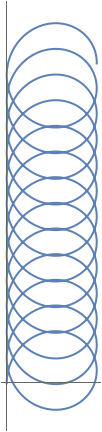
\includegraphics[keepaspectratio, scale=0.6]{fig/fig1.png}
    \caption{粒子の運動}
  \end{figure}


\end{enumerate}



\end{document}
